\documentclass[portrait,a0paper,fontscale=0.277]{baposter}

\usepackage{enumitem}
\setlist{nolistsep}

\usepackage[spanish]{babel}
\usepackage[utf8]{inputenc}
\usepackage{fontenc}
\usepackage{graphicx}
\usepackage{wrapfig}
%\usepackage{capt-of}
\usepackage{captdef}

\usepackage{tikz}
\usetikzlibrary{calc,automata,positioning,arrows}

\tikzstyle{line} = [draw, -latex]

%%%%%%%%%%%%%%%%%%%%%%%%%%%%%%%%%%%%%%%%%%%%%%%%%%%%%%%%%%%%%%%%%%%%%%%%%%%%%%%%
% Save space in lists. Use this after the opening of the list
%%%%%%%%%%%%%%%%%%%%%%%%%%%%%%%%%%%%%%%%%%%%%%%%%%%%%%%%%%%%%%%%%%%%%%%%%%%%%%%%
\newcommand{\compresslist}{%
\setlength{\topsep}{0pt}%
\setlength{\itemsep}{0pt}%
\setlength{\parskip}{0pt}%
\setlength{\parsep}{0pt}%
}


\newcommand{\Marca}[1]{{\bfseries\textcolor{green}{#1}}}
\newcommand{\MarcaErr}[1]{{\bfseries\textcolor{red}{#1}}}

\begin{document}
\begin{poster}
{ 
	background=plain,
	bgColorOne=white,
	borderColor=orange,
	linewidth=2pt,
	headershade=plain,
	headerColorOne=orange,
	boxshade=plain,
	boxColorOne=white,
	boxColorTwo=orange,
	textborder=roundedsmall,
	headerborder=open,
	headershape=smallrounded,
	headerheight=0.07\textheight,
	headerfont=\large\bf\textsc, %Sans Serif
	eyecatcher=true,
	columns=2
}
{} %\includegraphics[height=5.0em]{eji_logo} }
{ \Large\bf\textsc{Justificación, Redacción de Objetivos y Definición de Alcances en un Proyecto} }
{ \textsc\small{ \large{Bedrij Walter, Benitez Federico} \\ \footnotesize {wbedrij@gmail.com, federicobenitez2@gmail.com} } }  { \includegraphics[height=5.0em]{fich2} }

	\headerbox{Introducción}{name=intro,column=0,row=0}{
	
	La justificación del proyecto presenta los principales argumentos que permite convencer el porque el proyecto es necesario llevarlo a cabo como tambien verificar su viabilidad. 
La elaboracion de objetivos nos permite la planificacion y seguimiento del proyecto
Todo proyecto necesita cumplir determinados requisitos y se encuentra limitado por ciertas restricciones, esto queda defiido en el alcance del proyecto. 
	}

\headerbox{Desarrollo }{name=ana,column=0,span=1,below=intro}{

	\section*{Justificación}
	La Justificación permite tomar una decisión sobre si  el proyecto
debe avanzar a la siguiente etapa de desarrollo. 

Evaluar la viabilidad de una propuesta de proyecto.
implica:

\begin{itemize}\compresslist	
	\item Explicar las razones para el proyecto y los beneficios esperados.
	\item Describir el contexto relevante en términos de política, los negocios,
factores económicos y/o de programas.
	\item Describir las interdependencias con otros proyectos en caso de ser necesario.
	\item Indicar un aprendizaje previo relacionado con un aspecto de la justificación del proyecto, y explicar cómo ese aprendizaje podría ser beneficioso para el proyecto.
	\item Dar una evaluación de las medidas de éxito, basado en
criterios reconocidos.
	\end{itemize}

\section*{Objetivos: SMART}
\begin{description}
	\item[Specific (Específico)] Dejar explícito, para que no haya ambigüedad.
		\begin{itemize}\compresslist
			\item ¿Qué hacer? Acciones positivas.
			\item ¿Cuál será el resultado?
			\item ¿Por qué es importante?
			\item ¿Quién es el responsable?
			\item ¿Cuáles son los requerimientos y las restricciones?
		\end{itemize}
	\item[Measurable (Medible)]
	Definir criterios que indiquen que se logró el resultado esperado (o qué tan lejos estamos)
\item[Achievable (Alcanzable)]\hfill
	\begin{itemize}\compresslist
		\item ¿Se puede lograr con los recursos que disponemos?
		\item ¿Entendemos las restricciones?
		\item ¿Es posible y práctico?
	\end{itemize}
\item[Relevant (Relevante)]
	Cómo el objetivo se relaciona con el rol de cada miembro del equipo, y los objetivos de la organización.
	Los objetivos deben apoyarse mutuamente y no generar conflicto.
\item[Time-bound (Limitado en el tiempo)]
	Definir fechas límite.
	%¿Cuándo se completará?

\end{description}
	
	
\section*{Definir el Alcance} Es el proceso que consiste en desarrollar una descripción detallada del
proyecto y del producto. Se elabora a partir de los entregables principales, los supuestos y
las restricciones que se documentan durante el inicio del proyecto. Se analizan los riesgos, los
supuestos y las restricciones existentes, para verificar que estén completos; según sea necesario,
se irán agregando nuevos riesgos, supuestos y restricciones. 

	\begin{center}	
		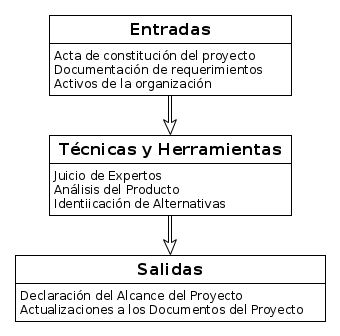
\includegraphics[width=.8\linewidth]{alcance}
	\end{center}
}

	\headerbox{Ejemplos}{name=ejemplo,column=1,span=1}{
	
	\section*{Motivación}
En el área del reconocimiento de patrones, un tópico de creciente interés
es el reconocimiento de gestos. Esta tarea consiste en la captura del movimiento
corporal de una persona mediante cámaras u otros dispositivos, y la
identificación de poses o movimientos particulares de la cabeza, mano, brazos, etc.
Los gestos reconocidos pueden ser empleados como entrada en el
control de equipamiento, ser traducidos a otra forma de información (p. ej.,
en la traducción de lenguaje de señas a voz). Migrar la interacción humano-computadora
a una manera más natural empleando la capacidad humana de
la gesticulación, permitiría el desarrollo de interfaces más efectivas y amigables
[DFAB03] [MA07].

El análisis y clasificación de gestos de la mano plantea algunas ventajas
respecto al análisis de otras partes del cuerpo. La mano facilita la representación
de un gran número de formas según la combinación de apertura y cierre
de los dedos, con un alto grado de libertad [EBN+07]. Estas características la
convierten en una herramienta de interacción muy efectiva, habiendo sido utilizada
en ambientes virtuales de navegación [Bow02], simulación quirúrgica
[LTCK03], generación de arte visual o música [vHB01, Tar05], entre otros.

   
    \section*{Objetivos: «SMARTER»}
\begin{description}
	\item[Specific (Específico)] dejar explícito, para que no haya ambigüedad.
		\begin{itemize}
			\item ¿Qué hacer? Acciones positivas.
			\item ¿Cuál será el resultado?
			\item ¿Por qué es importante?
			\item ¿Quién es el responsable?
			\item ¿Cuáles son los requerimientos y las restricciones?
		\end{itemize}
	\item[Measurable (Medible)]
	Definir criterios que indiquen que se logró el resultado esperado (o qué tan lejos estamos)
\item[Achievable (Alcanzable)]
	\begin{itemize}
		\item ¿Se puede lograr con los recursos que disponemos?
		\item ¿Entendemos las restricciones?
		\item ¿Es posible y práctico?
	\end{itemize}
\item[Relevant (Relevante)]
	Cómo el objetivo se relaciona con el rol de cada miembro del equipo, y los objetivos de la organización.
	Los objetivos deben apoyarse mutuamente y no generar conflicto.
\item[Time-bound (Limitado en el tiempo)]
	Definir fechas límite.
	%¿Cuándo se completará?
%revisar
\item[Evaluated (Evaluado)]
	Debe seguirse el progreso del objetivo.
	%Poder corregir.
\item[Rewarded (Recompensable)]
	Se vuelve un proceso de aprendizaje.
\end{description}

	
	\section* {Alcance} 
En este trabajo se presenta el diseño e implementación de un \Marca{sistema para
el reconocimiento} de signos manuales en \Marca{tiempo real}, mediante el procesamiento del flujo de video de una \Marca{cámara web} estándar en un \Marca{ambiente de
trabajo controlado}.

	
	}


  \headerbox{Conclusión}{name=questions,column=1,below=ejemplo}{
		\begin{itemize}\compresslist
			\item
		\end{itemize}
  }



  \headerbox{Referencias}{name=referencias,column=1,above=bottom}{
%%%%%%%%%%%%%%%%%%%%%%%%%%%%%%%%%%%%%%%%%%%%%%%%%%%%%%%%%%%%%%%%%%%%%%%%%%%%%%
    \bibliographystyle{ieee}
    \renewcommand{\section}[2]{\vskip 0.05em}
      \begin{thebibliography}{1}\itemsep=-0.01em
      \setlength{\baselineskip}{0.4em}

	  \bibitem{2004:GPM}
		\newblock{A Guide To The Project Management Body Of Knowledge (PMBOK Guides).}
		\newblock{Project Management Institute.}
		\newblock{2004.}
		
		\bibitem{2007:PMPJP}
		\newblock{Project Management:
Project Justification and
Planning.
}
		\newblock{Scottish Qualifications Authority.}
		\newblock{2007.}	
		
		 \bibitem{2012:FTG}
		 Graham Yemm.
		\newblock{FT Essential Guide to Leading Your Team: How to Set Goals, Measure Performance and Reward Talent.}
		\newblock{Pearson Education Limited.}
		\newblock{2012.}
		
		\bibitem{01:PFG}
		\newblock{Estructura básica para elaborar un Proyecto Finalde Graduación.}
		\newblock{Maestría en Administraciónde las Tecnologías de la Información. Universidad para la Cooperación Internacional.}
		\newblock{2012.}		
		
      \end{thebibliography}
   %\vspace{0.3em}
  }

\end{poster}
\end{document}
